\documentclass[tikz,border=10pt]{standalone}
\usepackage{amsmath}
\usepackage{amssymb}
\definecolor{mantis}{RGB}{0, 105, 62}
\begin{document}
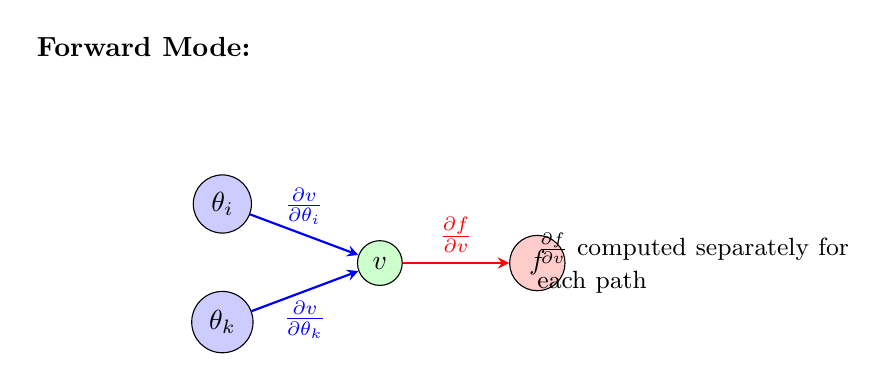
\begin{tikzpicture}[node distance=1.5cm, >=stealth]
    % Layer labels
    \node at (-1, 2) {\textbf{Forward Mode:}};
    
    % Nodes
    \node[draw, circle, fill=blue!20] (theta1) at (0, 0) {$\theta_i$};
    \node[draw, circle, fill=blue!20] (theta2) at (0, -1.5) {$\theta_k$};
    \node[draw, circle, fill=green!20] (v) at (2, -0.75) {$v$};
    \node[draw, circle, fill=red!20] (f) at (4, -0.75) {$f$};
    
    % Edges with labels
    \draw[->, thick, blue] (theta1) -- (v) node[midway, above] {$\frac{\partial v}{\partial \theta_i}$};
    \draw[->, thick, blue] (theta2) -- (v) node[midway, below] {$\frac{\partial v}{\partial \theta_k}$};
    \draw[->, thick, red] (v) -- (f) node[midway, above] {$\frac{\partial f}{\partial v}$};
    
    % Annotation
    \node[text width=4cm] at (6, -0.75) {\small $\frac{\partial f}{\partial v}$ computed separately for each path};
\end{tikzpicture}
\end{document}
